\chapter{Extending FABRIK}

As we've established in earlier chapters, having a good algorithm for inverse kinematics can be a helpful tool for motion planning of robotic manipulators. It can be used in two ways:

\begin{itemize}
  \item Finding joint parameters that allow the manipulator to reach the target, and then looking for a way to reach the position with i.e. RRT.\ In this case, we don't mind if the IK algorithm is slow, since we are only computing it once. However, we want guarantees that a solution is found, if one exists.
  \item Finding a path with respect to the end effector with a different method, and using IK to find collision-free positions for the remaining joints. In this case, the priority is speed of computation, since it needs to be recomputed repeatedly.
\end{itemize}

In either case, the algorithm needs to be extended with a way to respect joint limits, and avoid collisions with surrounding obstacles. Since our aim is to be able to control manipulators with a high DoF, the latter option is more interesting for us.

\section{Adding joint limits to FABRIK}

When considering joint limits, computing the positions of points in space, as the original algorithm does (recall~\ref{fig:fab}), is no longer sufficient; we need to consider what kind of joint we are currently dealing with, and what its orientation in space is.

Instead of points in space, we can use a complete kinematic model of our robot. This model, per DH convention, contains information about what joints and bodies the robot consists of and what parameters the joints are currently at. As a result, the model calculates the corresponding matrices of each joint with respect to the rest of the world. Whenever a joint is moved, transformation matrices of the joints affected by this change are recomputed.

Since we want the kinematic model to stay connected, we can no longer easily disconnect the joint from the remainder of the configuration. Instead, a virtual copy of the manipulator is created and rooted at the target position.

[picture]

This way, the joints of the copy serve as points for the forward reaching stage, and the original joints serve as points for the backward reaching stage. Rather than detaching the current joint and moving it to the desired position, joints are moved at each step to minimize the distance, while respecting joint limits.

Finding the right joint parameters can be done by expressing the desired position in spherical coordinates~\cite{spherical}.

Spherical coordinates are an alternative way to describe points in space, different from the standard cartesian $x, y, z$ coordinates. In a spherical coordinate system, each point is uniquely described as $(r, \theta, \phi)$, where $r$ is the radial distance, which is any nonnegative number; $\theta$ is the azimuth angle, standardly ranging $0 \leq \theta < 2\pi$ and $\phi$ is the polar angle, standardly ranging $0 \leq \phi \leq \pi$. The limits are flexible, and we can change them to better match the possible joint rotations. For instance the polar angle can also range $-\pi \le \theta < \pi$, in which case the same points will be expressed slightly differently.

Using the inverse transformation matrix of our current joint, we can express the desired position in cartesian coordinates with respect to the joint. Then, the position can be converted to polar coordinates using the following equations:
\begin{equation}
  r = \sqrt{x^2 + y^2 + z^2}
\end{equation}
\begin{equation}
  \theta = \atantwo(\frac{x}{y})
\end{equation}

\begin{equation}
  \phi = \sin(\frac{z}{r})
\end{equation}

If the current joint allows for extension, we can extend or retract it to the correct radial distance. Rotations can be adjusted according to the two angles.

As the two stages alter iteratively, the two models converge to each other. Since the transformation matrices need to be recomputed repeatedly, the whole process is slower than the original algorithm, but gains several advantages.

\begin{itemize}
  \item The algorithm for forward and backward reaching is exactly the same, hence, it can be reused and the code is less sensitive to changes in the kinematic model.
  \item Both stages automatically respect the joint limits, since the model itself can validate the performed movements.
  \item Every movement of the original kinematic model can realistically be performed. We can ensure that our manipulator is always in a consistent state throughout the algorithm, which allows us to visualize the whole algorithm, generate intermediate steps for the purposes of animation, or stop the algorithm at any moment.
\end{itemize}

The most straightforward way to enforce that the joint limits are respected is to simply clamp the computed angles. If the algorithm computes an angle outside the range of the current joint,
the joint is instead set to the nearest feasible angle.

\begin{figure}[h]
    \centering
    \begin{minipage}{\textwidth}
        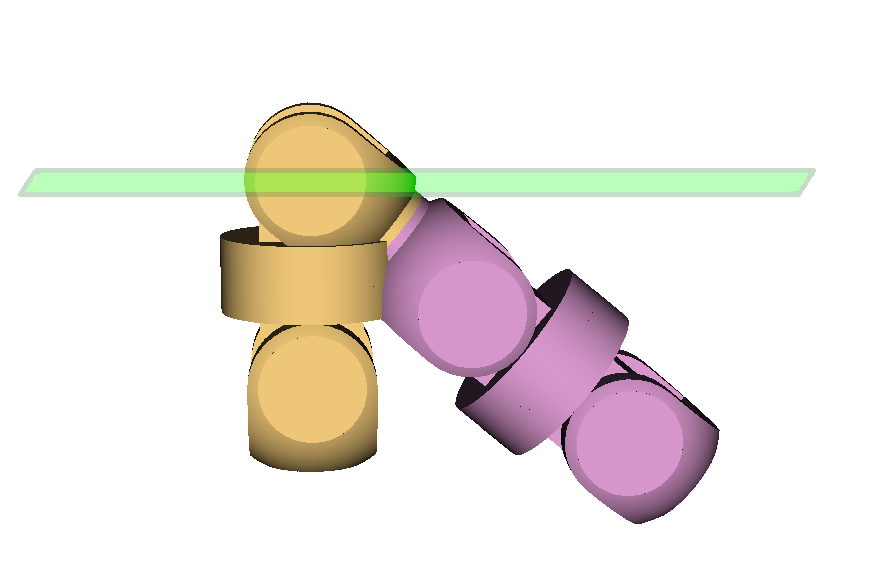
\includegraphics[width=.48\textwidth]{break_plane.png}
        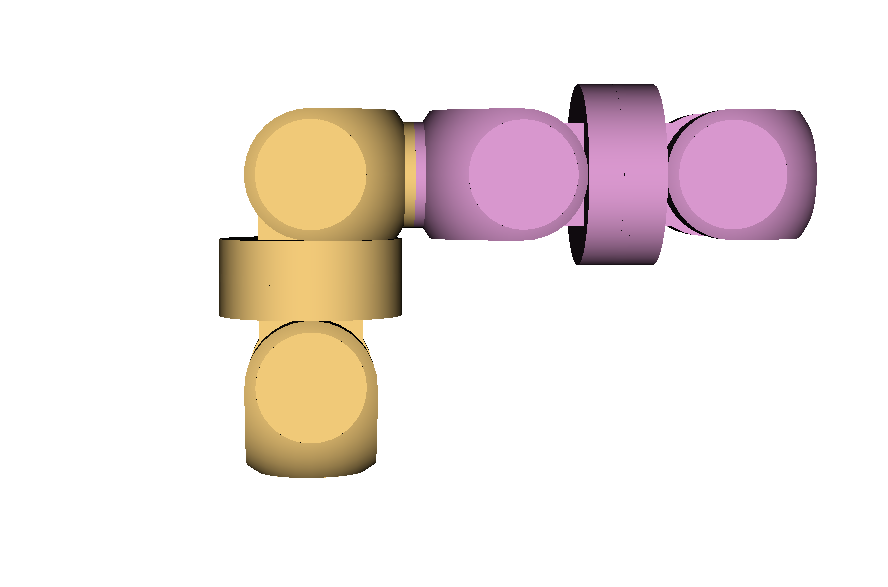
\includegraphics[width=.48\textwidth]{break_fixed.png}
    \end{minipage}
    \caption{The computed position violates the joint limit; the actual joint is clamped~\cite{Ondika2021thesis}.}\label{fig:break}
\end{figure}

While this limitation may prevent the algorithm from finishing in the current iteration, the other joints can make up for the limit and the manipulator is readjusted in the following iterations. In fact, as presented in~\cite{fabrik}, limitations on rotational joints can actually be helpful, in that more natural final poses are achieved.

The biggest problem we have to deal with comes when joints with only one degree of freedom are involved. Such joints can no longer rotate to an angle which minimizes the distance to the target joint, which means that we have to reason about the algorithm beyond the current joint for optimal results.

The optimal way to extend FABRIK to deal with this problem depends heavily on the build of the robot. Hence, in this part, the specifics of RoFI manipulators will be discussed; the core ideas may or may not translate to different manipulators.

Think back to the joints of the universal module (\ref{fig:um_rot}). When adapting the FABRIK algorithm to RoFI arms, we can treat each module as two joints. The joint between the two parts of a single module can only utilise the $\alpha$ or $\beta$ joint, hence, it is a simple rotational joint. As far as position of the next joint is concerned, the rotation of the $\gamma$ joint makes no difference. On the other hand, the joint between a universal module and the next component can utilise the $\gamma$ joint, and combine the two joints on the respective side to work as a ball joint and rotate in any direction. Passive modules or modules connected in a different direction can simply be viewed as a longer body between joints, and are not interesting for the algorithm.

The first idea that comes to mind may be to minimize the distance to the target joint position within the current limits. This is insufficient; if no special care is taken to account for joints that only have a single DoF, the manipulator will generally not reach the target.

The correct way to approach the problem is to align the one-dimensional joint in a way with the next target, so that only having one DoF is not limiting. Our implementation of FABRIK does exactly that: looking at the transformation created by the connection, the two DoF joint uses its mobility to place the next joint on the same plane as the target joint that follows it. As a result, the single DoF joint only needs to make a transformation in one plane, and the algorithm finds viable solutions to the constrained IK problem.

\begin{figure}[h]
    \centering
    \begin{minipage}{.6\textwidth}
        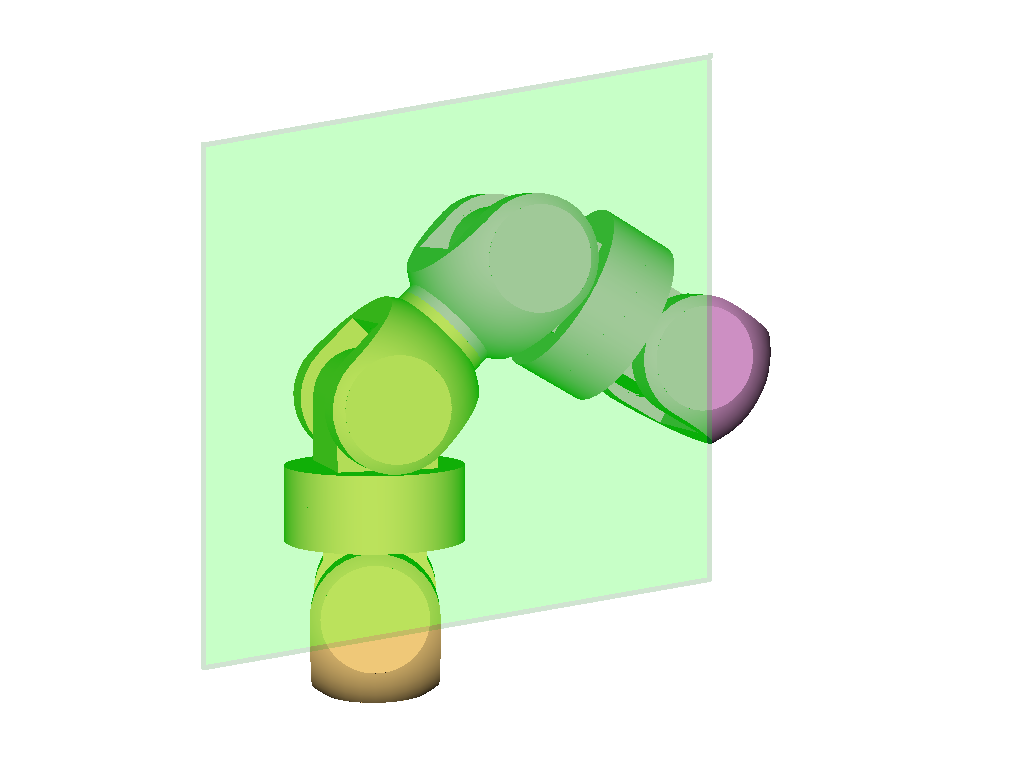
\includegraphics[width=\textwidth]{hinge_plane.png}
    \end{minipage}
    \caption{Visualization of the most common connection of modules: the first module is rotated so that the first joint of the second module lies in the target plane of the next joint~\cite{Ondika2021thesis}}\label{fig:hinge}
\end{figure}

Depending on the way the modules are connected, there are several cases that need to be dealt with in the implementation. A short summary:

\begin{itemize}
  \item Joint between parts of the same module: perform rotation along the X axis with respect to the current target
  \item Joint with Z-Z connection: perform rotation along the X axis with respect to the current target, rotation along the Z axis with respect to the following target
  \item Joint with Z-X connection: perform rotation along the X and Z axes with respect to the current target
  \item Joint with X-Z connection: perform rotation along Z with respect to the position of the current target, rotation along the X axis with respect to the following target
  \item Joint with X-X connection: perform rotation along the Z axis with respect to the current target
  \end{itemize}

Remeber that rotation along the joint's X axis is accomplished by the $\alpha$ and $\beta$ angles, while the rotation around Z corresponds to the $\gamma$ angle. The right angles are, as mentioned earlier, computed by fitting spherical coordinates to the possible movements of the joints: the azimuth angle (in radians) is clamped to $-\pi \le \theta < \pi$ to fit the $360\degree$ revolute Z joint, while the polar angle (in radians) is clamped to $-\frac{\pi}{2} \le \phi \le \frac{\pi}{2}$ to fit the $\left[-90\degree, 90\degree\right]$ X axis joint.

\section{Adding collision avoidance to FABRIK}

When discussing collision avoidance, the first question to ask is how to model the environment. Generally, we want to approximate objects in the workspace with simple geometric shapes: either polyhedra of choice, such as squares or pyramid shapes, or spheres. For simplicity and efficient representation, we shall choose the latter. Each joint of the manipulator shall be represented with a sphere\footnote{When considering RoFIbots, a single universal module can be modelled quite precisely with two adjacent spheres. With other types of robots, which may have longer bodies, rectangles or cylinders may be more suitable}. Without losing on generality, we can assume other objects in the workspace have also been approximated by the smallest sphere containing the entire shape.

For the moment, we will assume that the information about the workspace is complete; we know where all the objects are at the time we start the computation, and we have a complete model of the environment, created by a human or generated using an external camera.

One method for extending FABRIK with collision avoidance is presented here~\cite{fabrikAvoidance}. The authors propose that whenever a joint would be put in a position that causes a collision, the joint is put on a line between the current target and base of the arm, rather than the line between the current position and target. Then, if there is still a collision, a series of random rotations is used to avoid the obstacle.

If we were to compute IK only once, this method could prove useful. The method finds ways both around and between obstacles, and produces realistic poses. However, there are a few drawbacks:

\begin{itemize}
\item Since random rotations are used, there are no guarantees on the speed of convergence. As a result, as we can see from the authors' evaluation, the algorithm usually runs for around $0.1s$. We may be willing to wait that long once, but it is unimaginable to compute repeatedly.
\item Once again, no joint constraints are considered. When the current joint can only move in one plane, the initial guess of putting the joint as close to the base as possible is no longer well defined. In addition, random rotations in one direction may not lead to a solution due to hitting the joint limit, slowing the algorithm down even further.
\end{itemize}

In this thesis, a simpler approach to the collision avoidance problem within FABRIK is proposed.


During the forward reaching stage\footnote{Remember that in our extension, this moves the virtual copy of the manipulator, rooted in the target position.}, collisions are not checked. This allows the algorithm to find an approximate solution, but it is prone to collisions with surrounding objects.


During the backward reaching stage, the resulting position needs to be feasible. Hence, the new computed position for the joint is checked with the other objects in the workspace.

If the computed movement would cause a collision, a local limit is set on the current joint. A new joint rotation is computed within the limits set by nearby obstacles, and as a result, the manipulator gets as close to the desired position as possible, while avoiding a collision. The whole procedure is illustrated in Figure~\ref{fig:coll}.

\begin{figure}[h]
    \centering
    \begin{subfigure}{.24\textwidth}
      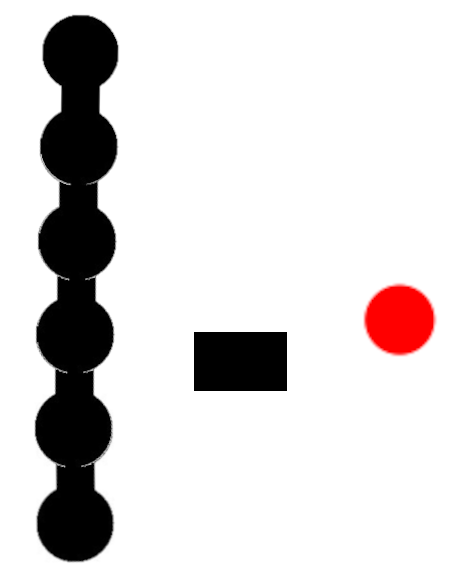
\includegraphics[width=0.9\textwidth]{coll_target.png}
      \caption{Initial position and target.}
    \end{subfigure}
    \begin{subfigure}{0.24\textwidth}
      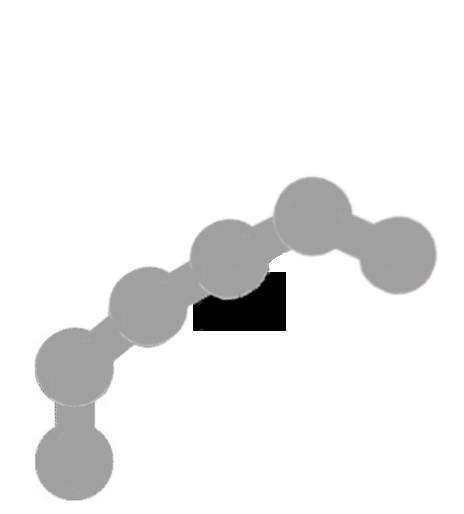
\includegraphics[width=0.9\textwidth]{coll_invalid.png}
      \caption{Solution from the first backward reaching stage.}
    \end{subfigure}
    \begin{subfigure}{.24\textwidth}
      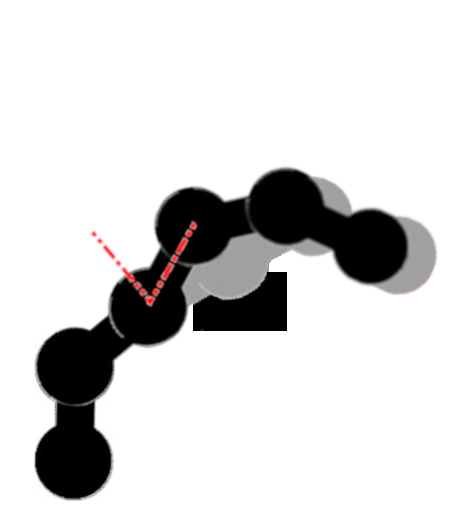
\includegraphics[width=0.9\textwidth]{coll_fixed.png}
      \caption{Collision is avoided by clamping the angle, but the target is not reached.}
    \end{subfigure}
    \begin{subfigure}{.24\textwidth}
      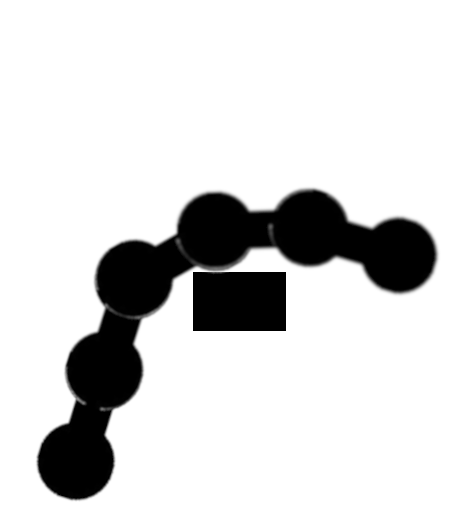
\includegraphics[width=0.9\textwidth]{coll_final.png}
      \caption{Final solution after a few iterations.}
    \end{subfigure}
    \caption{Illustration of FABRIK with simple collision avoidance.}\label{fig:coll}
\end{figure}
  
Note that compared to the aforementioned collision avoidance method, this one only works locally for each joint. As a result, it can get stuck in a local minimum, and not get over an obstacle. This is a disadvantage if we wanted to use it to immediately find a final solution; the algorithm could fail even though a solution exists. On the other hand, this behavior is desirable if we are using it to repeatedly compute incremental changes; the manipulator doesn't jump over obstacles when the actual movement is not directly possible. Additionally, the manipulator does not need complete knowledge of the environment, and we don't need to rely on randomness, which saves a lot of computational time.

As of now, we need to compare the new joint position with each other joint and each surrounding object in the workspace. Since other joints and obstacles are approximated with spheres, the collision check is very cheap: if the centers of two spheres are closer than the sum of their radii, the two spheres collide. However, checking every object is clearly asymptotically inefficient. Analog to doing lookup of strings or numbers in binary search trees, we would like to store our shapes in a structure that allows lookup with a logarithmic amount of comparisons.

A common structure for holding 3-dimensional information in robotics is the Octree~\cite{octree} -- this structure consists of squares, each of which is divident into 8 octants; subsquares of their parent. This structure allows easy lookup of data, but is not great for collision checking, since objects can span across various squares. In addition, modelling movement within an Octree can be difficult.

Hence, we opt for the data structure more commonly used in video games -- Axis Aligned Bounding Box Trees, AABB for short~\cite{aabb}. An AABB is a binary tree where shapes are stored in the leaves, and each inner node serves as the bounding box of its children. The bounding boxes are, as the name suggests, axis aligned -- we define them with standard $x, y, z$ dimensions and do not consider varying rotations. Unlike octrees, nodes in the AABB are of varying size, see Figure~\ref{fig:aabb}.

\begin{figure}[h]
  \centering
  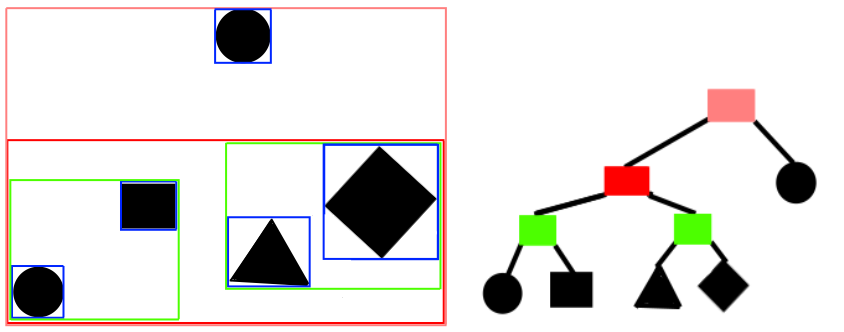
\includegraphics[width=0.8\textwidth]{aabb.png}
  \caption{Obstacles in space with the corresponding bounding boxes, and the inner structure of the AABB tree holding them.}\label{fig:aabb}
\end{figure}

The internal workings of an AABB are best explained using the actual operations. When the first shape is inserted into an AABB, a new node is created with a bounding box containing the shape. When inserting further shapes, the structure first chooses what leaf it shall become a sibling to, based on specified criteria.
Once a sibling has been chosen, the following operation proceeds:

\begin{enumerate}
\item Create a new parent node in place of the sibling leaf.
\item Make the sibling leaf a child of the new node.
\item Make the new leaf the other child of the new node.
\item Resize the parent node bounding box so that both shapes fit into it.
\item Recursively proceed to the root, increasing all the bounding boxes if necessary.
\end{enumerate}

A common heuristic for choosing where to insert the new leaf is to descend the tree starting from the root, always choosing the child in that will lead to smaller resizing of the tree. When we perform random insertions, the tree balances itself out quite evenly.

The payoff for building the data structure in this way is efficient lookup. When we need to check if a shape would collide with any other shape already in the structure, we do not need to compare it to every leaf. Instead, collision lookup proceeds from the root and only enters nodes with bounding boxes that collide with our shape. If the shape does not collide with either of the bounding boxes, we know that it does not collide with the leaves either, as the leaf shapes are contained within the nodes by definition. If it does collide with a bounding box, we check for the children, potentially getting to leaf nodes. Then, finally, collision with the actual object is checked.

\begin{wrapfigure}{r}{0.4\textwidth}
  \centering
  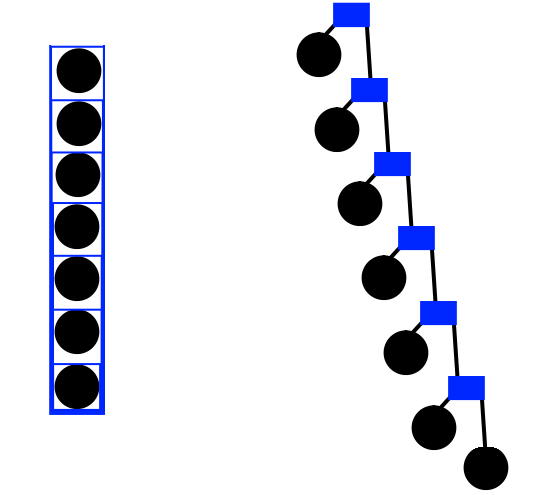
\includegraphics[width=0.4\textwidth]{degenerate.png}
  \caption{When objects are aligned and added one by one, a degenerate tree can be created.}
\end{wrapfigure}

In practice, the insertion heuristic performs well, and the \textit{expected} number of comparisons is significantly smaller than when trying to compare all the objects. However, the heuristic itself does not guarantee logarithmic depth; there is a case which leads to a degenerate tree. This tree can come to exist if all the objects are aligned and added to the tree starting from one end. Then, if we are checking collisions of an object close to the deepest leaf of our tree, the amount of comparisons is equal to the number of objects. This problem could be mitigated by adding balancing rotations to the tree, but in most cases, the extra work is unnecessary.

Now, how do we apply these trees to our problem? Assuming we already have a model of the environment, building the AABB is a simple matter of inserting each shape into it. To represent movement within an AABB, we need to erase the corresponding shape and then reinsert it at the new position.

Recall that in each backward iteration of FABRIK, we want to check if the current joint can be placed at the computed position. The invariant of our algorithm is that each joint has a corresponding sphere in the AABB, and the kinematic model of the manipulator has a pointer to it.

Therefore, we extend the backward FABRIK iterations by first erasing the joint leaves from the AABB. Then, when we compute a position for the joint, we check if it causes a collision with AABB lookup. If it does, we readjust it accordingly. When a reachable position for the joint is found, the joint is fixed for the remainder of the iteration, and the corresponding sphere is reinserted into the AABB. While it may seem that we've done a lot of unnecessary work, we can now guarantee that none of the joints will collide with other parts of the manipulator, or any static obstacle, without exhaustively checking all of them.

The difference may not be felt when all the obstacles are spheres, but it is particularly noticeable when we generalise obstacles to arbitrary shapes. Then, a collision check can be quite an expensive operation, and avoiding unnecessary checks with cheap bounding box comparisons can save a lot of computational time.
